\chapter{Grundlagen}

\section{Entwicklung mit Ruby on Rails}

2004 arbeitete der dänische Programmierer David Heinemeier Hansson an der Umsetzung eines webbasierten Projektmanagement-Tools mit dem Namen Basecamp\footnote{Projekt-Homepage: \href{http://basecamphq.com/}{http://basecamphq.com/}}. Die bei der Realisierung des Projektes umgesetzten Teilkomponenten extrahierte er später und veröffentlicht sie 2005 als Framework unter dem Namen Ruby on Rails.
Ruby on Rails basiert dabei auf der objektorientierten Programmiersprache Ruby und ermöglicht die schnelle Entwicklung von Webanwendungen nach dem MVC-Paradigma (Kapitel sec:mvc).
\newline
6 Jahre später (die zahlreiche Änderungen und Verbesserungen am Framework ermöglichten) beschreibt sich das Ruby on Rails-Projekt selbst mit folgenden plakativen Worten:
\begin{quote}
Ruby on Rails is an open-source web framework that’s
optimized for programmer happiness and sustainable
productivity. It lets you write beautiful code by
favoring convention over configuration. \cite[vgl.][]{RailsStatement}
\end{quote}

Diese subjektive Aussage der Rails-Kernentwickler bezieht sich dabei auf viele Ansätze und Entwicklungsabläufe, die innerhalb des Frameworks umgesetzt werden.
Im folgenden Abschnitt sollen die mit dieser Aussage angedeuteten wichtigsten Prinzipien, Paradigmen und Programmierabläufe des Frameworks zusammengefasst werden, um auf dieser Grundlage eine nichtfunktionale Betrachtung der Rails WCMS in Kapitel 4 zu ermöglichen. Auf die Themen Rest (Kapitel \ref{grundrest}) und Middleware (Kapitel \ref{grundrack}) wird dabei ausführlicher eingegangen, um für die in Kapitel 5 umgesetzten Lösungsvorschläge entsprechendes Vorwissen zu schaffen.
\newline
\newline
Für eine umfassende Einführung in Rails werden \cite{RubyMetaprogramming2010} und \cite{EnterpriseRails} empfohlen.

\subsection{Don't-Repeat-Yourself (DRY)}
Zur Optimierung der Entwicklungvorgänge innerhalb des Frameworks propagiert Rails den Grundsatz des DRY (Don't-Repeat-Yourself). Dabei sollen Redundanzen, d.h. die wiederholte Angabe identischer Informationen jeglicher Art vermieden werden. So kann sichergestellt werden, dass sich Änderungen an einer zentralen Stelle im System (z.B. Quellcode) in der gesamten Anwendung auswirken und Duplikate nicht mehrfach angepasst werden müssen.
\subsection{Convention over Configuration}
Viele Web Frameworks müssen vor ihrer Nutzung erst mit Hilfe zahlreicher Konfigurationsdateien und Parametereinstellungen zu einem lauffähigen Gesamtsystem zusammengebaut werden\footnote{Rails bezeichnet diese Art der Frameworks mit ihrem Konfigurations-Overhead oft als \emph{enterprisy}. Dies bedeutet jedoch nicht, das Rails für Anwendungsumsetzungen im Enterprise-Bereich ungeeignet ist. \citep[vgl.][]{enterprisy}.}. Abbildung \ref{spring} zeigt beispielhaft solch eine Konfigurationsdatei innerhalb des Java Application Frameworks Spring\footnote{Projektseite: \href{http://www.springsource.org/}{http://www.springsource.org/}}:

\lstinputlisting[label=spring,language=xml, caption=Konfigurationsdatei im Java Spring Framework]{code/spring.xml}
Um diesen zusätzlichen und zeitraubenden Aufwand vor der eigentlichen Arbeit mit einem Framework zu vermeiden, definiert Rails zahlreiche Konventionen, die es erlauben, sofort mit der Entwicklungsarbeit zu beginnen. U.a. werden folgende Festlegungen getroffen:

\begin{itemize}
\item
Informationen zur Datenbankverbindung der Anwendung müssen in der Datei database.yml im Unterordner config hinterlegt werden
\item
Der Klassenname eines Domainenmodells wird im Singular erwartet, der dazu korrespondierende Tabellename in der Datenbank hingegen im Plural z.B. Domainenmodell Project => Datenbanktabelle projects
\item
Der Primärschlüssel in einer Datanbanktabelle muss vom Typ Integer sein und den Namen ID besitzen
\item
Rails erwartet eine definierte Ordnerstrukur für Controller, Domainmodell und Views\footnote{Eine Erklärung zu Model-View-Controller folgt in Abschnitt \ref{sec:mvc}}
\end{itemize}
Für den produktiven Einsatz des Frameworks müssen diese daher erlernt und akzeptiert werden, was dazu führt, dass Rails häufig als \emph{opinionated software\footnote{Eine ausführliche Stellungnahme von Rails-Erfinder David Heinemeier Hansson zu diesem Thema gibt es unter: \href{http://www.linuxjournal.com/article/8686}{http://www.linuxjournal.com/article/8686}}} (starr- und eigensinnige Software) bezeichnet wird.

Ein Abweichen von den definierten Konventionen ist jederzeit möglich, erhöht jedoch den Aufwand des Entwicklers.

\subsection{Model-View-Controller (MVC)}
\label{sec:mvc}
Für Software-Designer ist es  eine gebräuchliche Technik, komplexe Software-Systeme durch Schichtenbildung in einzelne Bestandteile zu zerlegen \citep[Kapitel 1]{FowlerPatterns}. Das Ruby on Rails Framework baut ebenfalls auf einem Mehr-Schichten-Architektur-Modell auf. Zusätzlich kommt eine für das Rails-Framework spezifische Implementierung des bereits 1979 von dem Norweger Trygve Mikkjel Heyerdahl entwickelten Model-View-Controller-Paradigmas zum Einsatz\footnote{In der Fachliteratur wird das MVC-Paradigma häufig auf die Schichtenarchitektur einer Anwendung übertragen \cite[S. 544 ff.]{objekt}. Tatsächlich betrifft MVC in seiner  ursprünglichen Form nur die Präsentationsschicht einer Webanwendung.}.
Abbildung \ref{fig:mvcimage} charakterisiert den Ablauf einer Anfrage (Request) an eine Rails-Anwendung innerhalb des Client-Server-Modells sowie die Komponenten Model, View und Controller, die eine logische Trennung der Anwendung in verschiedene Verantwortungsbereiche ermöglichen:

\begin{figure}[!h]
\begin{center}
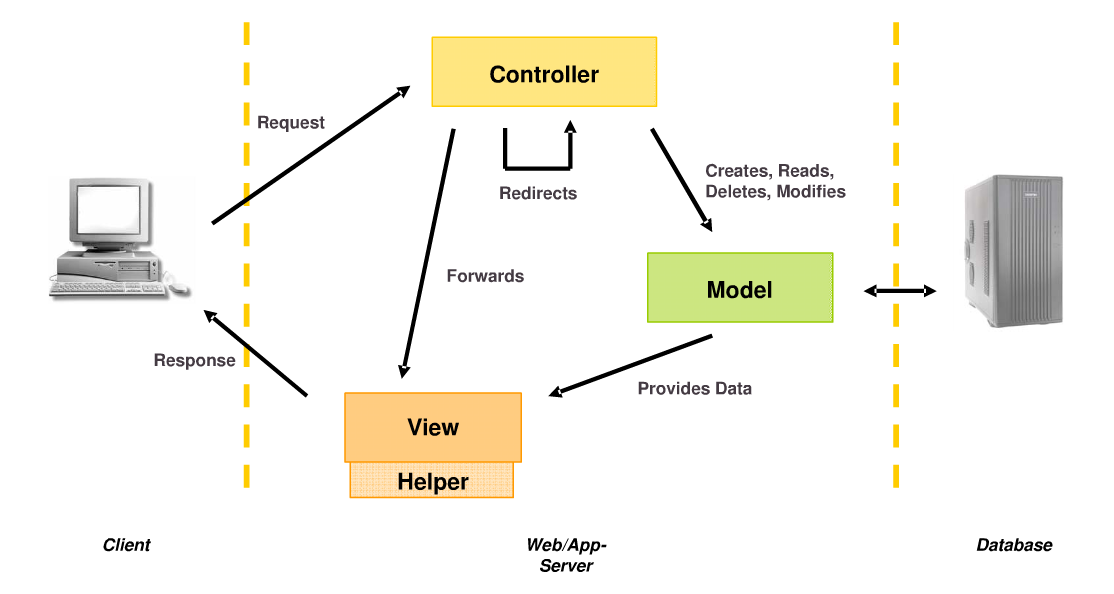
\includegraphics[scale=0.4]{images/analyse/mvc.png}
%\caption{Nutzung verschiedener Programmiersprachen auf Servern}{Quelle: \citep{w3techs}}


\caption[Verarbeitung einer Anfrage innerhalb des Rails-Frameworks]{Verarbeitung einer Anfrage (Client-Server-Modell) innerhalb des Rails-Frameworks. Quelle: \citep[Seite 6]{railsmvc}}
\label{fig:mvcimage}
\end{center}
\end{figure}

\begin{enumerate}
\item
Anfrage eines Clienten
\item
An Hand der im Rails-Routing definierten Einträge wird die Anfrage eines Clienten an den registrierten Controller weitergeleitet
\item
Der Controller steuert den Ablauf innerhalb der Anwendung. Dabei greift er über ein Model auf benötigte Daten in einem Speicher (z.B. relationale Datenbank) zu und stellt diese dem View-Layer zur Verfügung. Es ist auch möglich, dass der Controller die Anfrage an einen anderen Controller weiterleitet (Redirects). Im Gesamtkonzept von Rails enthält der Controller die Programmlogik der Anwendung.
\item
Als Model werden in Rails Ruby-Klassen bezeichnet, die einen Zugriff auf relationale Datenbanken oder andere Datenspeicher ermöglichen \citep[vgl.][]{Rails2}. Es bildet innerhalb der Anwendung die zugrundliegende Datenstruktur ab.
%\citep[vgl.][]{Rails2}
\item
Der View-Layer (Sicht- oder Darstellungsschicht) bereitet die durch den Controller zur Verfügung gestellten Daten in der angeforderten Darstellungsform auf und gibt das Ergebnis der Anfrage aus. So wird je nach spezifiziertem Format z.B. eine HTML- oder XML-Datei erzeugt. Ein View repräsentiert somit die Darstellung einer bestimmten Datenstruktur (Model).
\item
Das Ergebnis der Anfrage (die Ausgabe des View) wird vom Framework an den Server übermittelt und von dort an den Clienten ausgeliefert (Response). Der Kommunikationsprozess mit dem Rails-Framework ist damit abgeschlossen.
\end{enumerate}



\subsection{REST}
\label{grundrest}
Innerhalb einer Web-Applikation erfolgt der Austausch zwischen Server und Client durch die Nutzung des HTTP-Protokolls. Dabei wird eine Anfrage (Request) an einen Server geschickt, bearbeitet und eine entsprechende Antwort (Response) mit den angeforderten Inhalten zurückliefert. Ein Großteil der Webanwendungen interpretiert dabei die im HTTP-Protokoll definierten Methoden GET und POST:

\begin{description}
\item[GET]
Anforderung an den Server, eine über die Adresszeile des Browsers angegebene Ressource zurückzuliefern. Es können zusätzlich Argumente an die angeforderte URL angehängt werden.
\item[POST]
Mit Hilfe dieser Methode ist es möglich, große Datenmengen aus z.B. Formularen an einen Webserver zu verschicken. Die übergebenen Informationen werden dabei im sogenannten Body der Anfrage codiert mitverschickt und somit im Vergleich zu GET nicht in der URL sichtbar\footnote{Ein Post-Request findet vor allem bei der Übermittlung von Formularen innerhalb eines Browsers Verwendung.}.
\end{description}


REST, ein Akronym für \textbf{RE}epresentational \textbf{S}tate \textbf{T}ransfer, erweitert die in  traditionellen Webanwendungen üblichen GET und POST um die ebenfalls im HTTP-Standard enthaltenen Methoden PUT und DELETE:
\begin{comment}
\begin{description}
\item[GET]
Abfrage einer Ressource unter der angegebenen URL mit  anschließender Darstellung
\item[POST]
Erstellung einer neuen Ressourcen an Hand der in der Anfrage übermittelten Daten, Realisierung durch Formulare auf Clientseite
\item[PUT]
Überschreiben der angeforderten Ressource mit den in der Anfrage neu übermittelten Daten
\item[DELETE]
Löschen der beschriebenen Ressource
\end{description}
\end{comment}

\begin{description}
\item[PUT]
	Die Verwendung der PUT-Methode zeigt die Neuanlage der in einer	Anfrage spezifizierten Ressource an
\item[DELETE]
	Die Verwendung dieser Methode signalisiert dem Server, die angegebene Ressource auf dem Server zu löschen.
\end{description}
Da aktuelle Browser nur GET- und POST-Anfragen zuverlässig unterstützen, müssen entsprechende Anfragen zum Löschen und Verändern einer Ressource mit Hilfe von zusätzlichen Attributen in der Anfrage simuliert werden\footnote{Das Rails Framework fügt  innerhalb von Formularen automatisch einen versteckten Parameter \emph{\_method} in die Anfrage, die den Namen der gewünschten HTTP-Metode (DELETE oder PUT) enthält. Im Framework wird dieser Parameter ausgelesen und ein entsprechendes Routing zur geforderten Controller-Action eingeleitet.}. Das folgende Beispiel stellt das von Rails definierte Standard-Routing einer als \emph{restful} angelegten Ressource Projekt dar\footnote{REST wird nicht über einen entsprechend formulierten Standard definiert. Vielmehr kann es als Programmierparadigma innerhalb von Web-Anwendungen verstanden werden, die eine Ansammlung von Best-Practices darstellen \cite{restful}.}.

\begin{table}[!h]
\caption{Rails Routing der Rest-Ressource Projekt}
\center
\begin{tabular}[!ht]{|p{2cm}|p{3cm}|p{3cm}|p{6cm}|}
\hline
HTTP-Methode & Anfragepfad & Ausgelöste Aktion im Controller & Wirkung\\
\hline
GET	& /projects & index & Anzeige aller vorhandenen Projekte\\
\hline
GET	& /projects/new	& new &	Anzeige eines HTML-Formulars zum erstellen eines neuen Projektes\\
\hline
POST & /projects & create & Erstellt ein neues Projekt mit den übermittelten Daten\\
\hline
GET & /projects/:id &	show &	Anzeige eines Projektes mit der zugeordneten ID\\
\hline
GET	& /projects/:id/edit & edit & Anzeige eines HTML-Formulars zum Bearbeiten eines bestehenden Projektes\\
\hline
PUT	& /projects/:id &	update & Aktualisierung eines bestimmten Projektes mit den übermittelten Daten\\
\hline
DELETE & /projects/:id &	destroy &	Löschung des Projektes mit der angegebenen ID\\
\hline
\end{tabular}
\end{table}

\begin{table}[!ht]
\caption{Vergleich zwischen Rest-konformen und klassischen Rails-URL's}
\label{tab.restnonrest}
\center
\begin{tabular}[!ht]{|l|l|l|}
\hline
Aktion & normale URL & 	REST URL in Rails \\
\hline
show &	/projects/show/12 &	/projects/12 \\
\hline
delete & /projects/destroy/123 & /projects/123 \\
\hline
update & /projects/update/123 &	/projects/123 \\
\hline
create & /projects/create & /projects \\
\hline
\end{tabular}
\end{table}

Tabelle \ref{tab.restnonrest} zeigt noch einmal die Trennung zwischen Ressource und Aktion innerhalb einer in Rails definierten REST-Ressource Projekt. Eine ausführliche Beschreibung von REST und dessen Realisierung liefert \cite{restful}.

\newpage
\subsection{Rack und Middleware}
\label{grundrack}
Rails ist innerhalb der Ruby-Gemeinde nicht das einzigste existierende Webframework. Mit den Projekten Sinatra\footnote{Projektseite: \href{http://www.sinatrarb.com/}{http://www.sinatrarb.com/}}, Merb\footnote{Projektseite: \href{http://www.merbivore.com/}{http://www.merbivore.com/}}, Camping\footnote{Projektseite: \href{http://camping.rubyforge.org/}{http://camping.rubyforge.org/}} und Ramaze\footnote{Projektseite: \href{http://ramaze.net/}{http://ramaze.net/}} stehen weitere Alternativen mit unterschiedlichen Ansätzen und Funktionsumfängen zur Verfügung.
Bei der Implementierung dieser Frameworks müssen Entwickler wiederholt Adapter\footnote{} (Handler) zur Ansteuerung verschiedener Webserver entwickeln. Durch Rack\footnote{Projektseite: \href{http://rack.rubyforge.org/}{http://rack.rubyforge.org/}}, einem Ruby Webserver Interface, lässt sich die wiederholte Implementierung solcher Adapter in den einzelnen Frameworks vermeiden.
\begin{figure}[!h]
\begin{center}
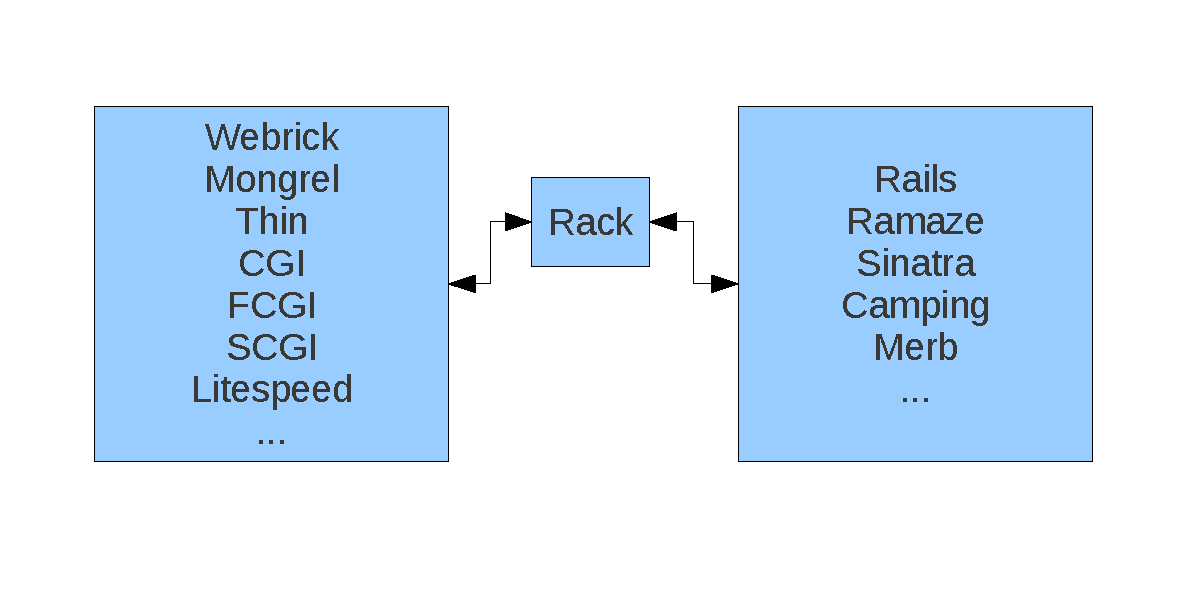
\includegraphics[scale=0.47]{images/rack/rack.pdf}
\caption{Rack als Vermittler zwischen Server und Ruby-Webframeworks}
\label{rackschema}
\end{center}
\end{figure}


Damit Server und Frameworks untereinander kommunizieren können, muss eine Rack-Anwendung bestimmte Methoden implementieren und ein bestimmtes Rückgabeformat einhalten. An Hand des Beispiels in \ref{rack} sollen diese formalen Kriterien beschrieben werden:

\lstinputlisting[label=rack,language=Ruby, caption=Beispiel für eine einfache Rack-Anwendung]{code/rack.rb}

\begin{description}
\item[Zeile 6-8]\mbox{~}\\*
Initialisierung der Rack-Anwendung MyRackApp unter Angabe eines zuvor übergebenen Namen (\emph{Rack} in Zeile 15).
\item[Zeile 10-12]\mbox{~}\\*
Implementierung der für eine Rack-Anwendung notwendigen Methode \emph{call}. Diese wird vom Webserver beim Start einer Anfrage aufgerufen und muss als Antwort (Rückgabewert) einen Ruby-Hash mit den folgenden Informationen zurückliefern:
\begin{description}
\item[Status]\mbox{~}\\*
Angabe des HTTP-Statuscode, \emph{200} bedeutet in diesem Beispiel eine erfolgreiche Ausführung der Anfrage am Server\footnote{Die HTTP-Statuscodes sind im HTTP-Protokoll definiert und können u.a. unter folgender Quelle eingesehen werden: \href{http://www.w3.org/Protocols/rfc2616/rfc2616-sec10.html}{http://www.w3.org/Protocols/rfc2616/rfc2616-sec10.html}}
\item[Header]\mbox{~}\\*
Angabe von im HTTP-Protokoll definierten Header-Informationen,  im Beispiel wird ein einfaches Textdokument (\emph{text/plain}) zurückgeliefert
\item[Response]\mbox{~}\\*
Die Antwort der Rack-Anwendung, im Beispiel wird ein String \emph{Hello Rack!} an den Server übergeben und von diesem ausgeliefert.
\end{description}

Beim Aufruf der Methode \emph{call} (Zeile 15) übergibt der Server eine Variable \emph{env}, die alle wichtigen Informationen über die Serverumgebung und Anfrageparameter enthält.
\item[Zeile 15]\mbox{~}\\*
Start des Mongrel Webservers und Initialisierung der Rack-Anwendung \emph{MyRackApp}.
\end{description}

Bei einem Aufruf der Adresse \emph{localhost:3001} in einem Browser wird vom gestarteten Mongrel-Server der Rückgabewert der Methode \emph{call} ausgegeben (Abb. \ref{rackoutput}).

\begin{figure}[!ht]
\begin{center}
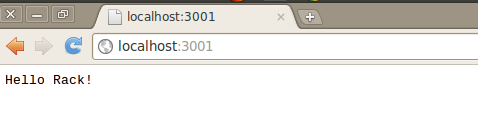
\includegraphics[scale=0.6]{images/rack/outputrack2.png}
\caption{Ausgabe der Rack-Anwendung MyRackApp im Browser}
\label{rackoutput}
\end{center}
\end{figure}

Durch die Nutzung von Rack ergeben sich im Bereich der Ruby Webframeworks folgende Vorteile:

\begin{itemize}
\item
Vereinfachung der Webframework-Entwicklung: Ein Framework, das Rack unterstützt, kann sofort von allen anderen rack-unterstützenden Webservern verwendet werden.
\item
Vereinfachung der Serverentwicklung: Ein rack-unterstützender Server kann sofort mit allen rack-basierten Webframeworks eingesetzt werden.
\item
Keine Codeduplizierung durch wiederholte Entwicklung von Server-Adaptern innerhalb der verschiedenen Ruby Webframeworks
\item
Rack beinhaltet Handler für die meist verbreitesten Webserver in Ruby (Abbildung \ref{rackschema})
\end{itemize}


Darüber hinaus ist es  möglich, einzelne Rack-Anwendungen hintereinander zu schalten und so ein Filtersystem für ankommende Anfragen und ausgehende Antworten vor dem eigentlichen Webframework zu realisieren.
Diese Anwendungen werden Rack-Middlewares genannt und können in einer Rails-Anwendung in der Startkonfiguration des Frameworks eingebunden werden. So kann das Ein- und Ausgabeverhalten des Railsframeworks gezielt verändert werden, da die einzelnen Rack-Anwendungen entscheiden, ob der nächste Filter (die nächste registrierte Rack-Middleware) oder eine vorzeitige Anwort an den Server geschickt werden soll.

%\lstinputlisting[label=middlewarestack,language=Ruby, caption=Registrierung verschiedener Middlewares in einer Rails 3 Anwendung]{code/middleware.rb}
Das Rails-Framework steht selbst am Ende der Filterliste und ist im Kontext von Rack selbst als Rack-Anwendung eingebunden (Abb. \ref{rackmiddlewares}). Eine detaillierte Beschreibung von Rack und der Einrichtung eines komplexen Filtersystems\footnote{Rack stellt häufig verwendete Middlewares für verschiedene Aufgabenbereiche zur Verfügung. Die Projektseite ist unter folgender Adresse verfügbar: \href{https://github.com/rack/rack-contrib}{https://github.com/rack/rack-contrib}} in einer Rails-Anwendung liefern \cite{rack} und \cite{railsguiderack}.
\begin{figure}[!ht]
\begin{center}
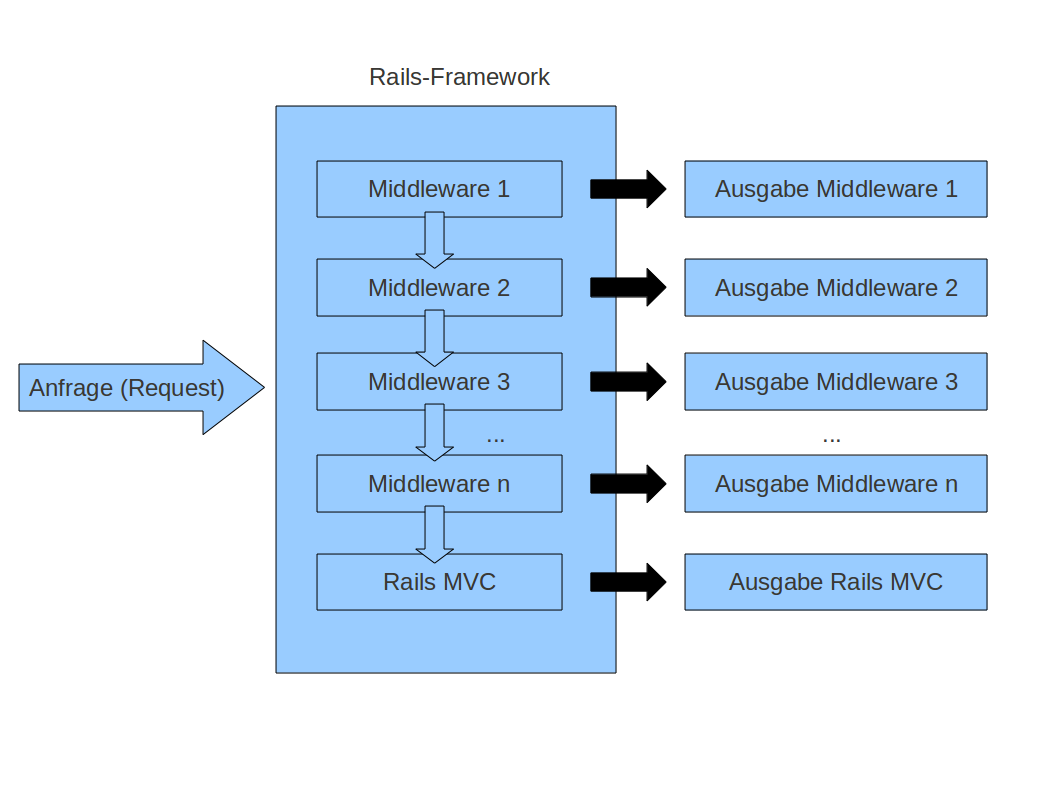
\includegraphics[scale=0.5]{images/rack/middlewares.png}
\caption{Möglichkeiten der unterschiedlichen Rückgabewerte durch Rack Middlewares und Rails}
\label{rackmiddlewares}
\end{center}
\end{figure}
\subsection{Generatoren}
\label{sec:railsgeneratoren}
Das Ruby on Rails Framework unterstützt mit Hilfe sogenannter Generatorskripte die automatische Erzeugung von funktionsfähigem Quellcode. Der folgende Scaffold-Generator\footnote{Scaffold kann in diesem Zusammenhang mit dem Wort Grundgerüst übersetzt werden.} erstellt z.B. nach dessen Initialisierung ein komplett funktionsbereites Codegerüst für die in Rails benötigten MVC-Komponenten einer Ressource \emph{Projekt}.

%\begin{lstlisting}[caption=Aufruf des Generators zur Erstellung einer MVC-Ressource Projekt]
%rails g scaffold project name:string description:text
%\end{lstlisting}

\lstinputlisting[label=scaffold,language=Ruby, caption=Aufruf des Generators zur Erstellung einer MVC-Ressource Projekt mit Ausgabe der erstellten Dateien]{code/scaffold.txt}

\section{Web Content Management, Content Life Cycle und Web-Publishing}
\label{sec:webpublishing}
Der Anstieg von digitalen Informationen und Content\footnote{
\glqq Unter dem Begriff des \flqq Contents\frqq~ werden alle Inhalte verstanden, die in einem CMS verwaltet werden und die im engeren Sinne für die Erstellung von Dokumenten und Publikationen verwendet werden. Darunter fallen alle textuellen und (audio-)visuellen Informationen [..] \citep[S. 297]{TechnischeDok}
} erfordert innerhalb der einzelnen Unternehmen ein immer umfangreicheres und zielgerichteteres Management. Der so entstandene Begriff des Content Management wird dabei u.a. von Berechtenbreiter mit folgenden Worten umschrieben:
\begin{quote}
Content Management beschreibt die Planung, Verwaltung, Steuerung und Koordination aller Aktivitäten, die auf den Content und dessen Präsentation in Unternehmen abstellen \cite{Berchtenbreiter}.
\end{quote}

Im Bereich der internet-basierten Web-Sites und Internet-Portale hat dies zur Herausbildung des Web Content Managements geführt \citep[][S. 3]{ecm}. Die dort verwendeten Softwarelösungen (WCMS) streben dabei die Implementierung des Content Life Cycle (Inhaltslebenszyklus) ab, der als stark vereinfachtes Prozessmodell alle wichtige Phasen\footnote{Die Content-Nutzung durch den Endanwender (Internetseitennutzer) findet innerhalb des Content Life Cycle keine Beachtung.}, die ein beliebiger Inhalt (Informationsträger) während seiner Existenz durchläuft, abbildet \citep[S.303]{TechnischeDok}. Im folgenden sollen diese Teilprozesse erläutert werden:

\begin{figure}[!ht]
\begin{center}
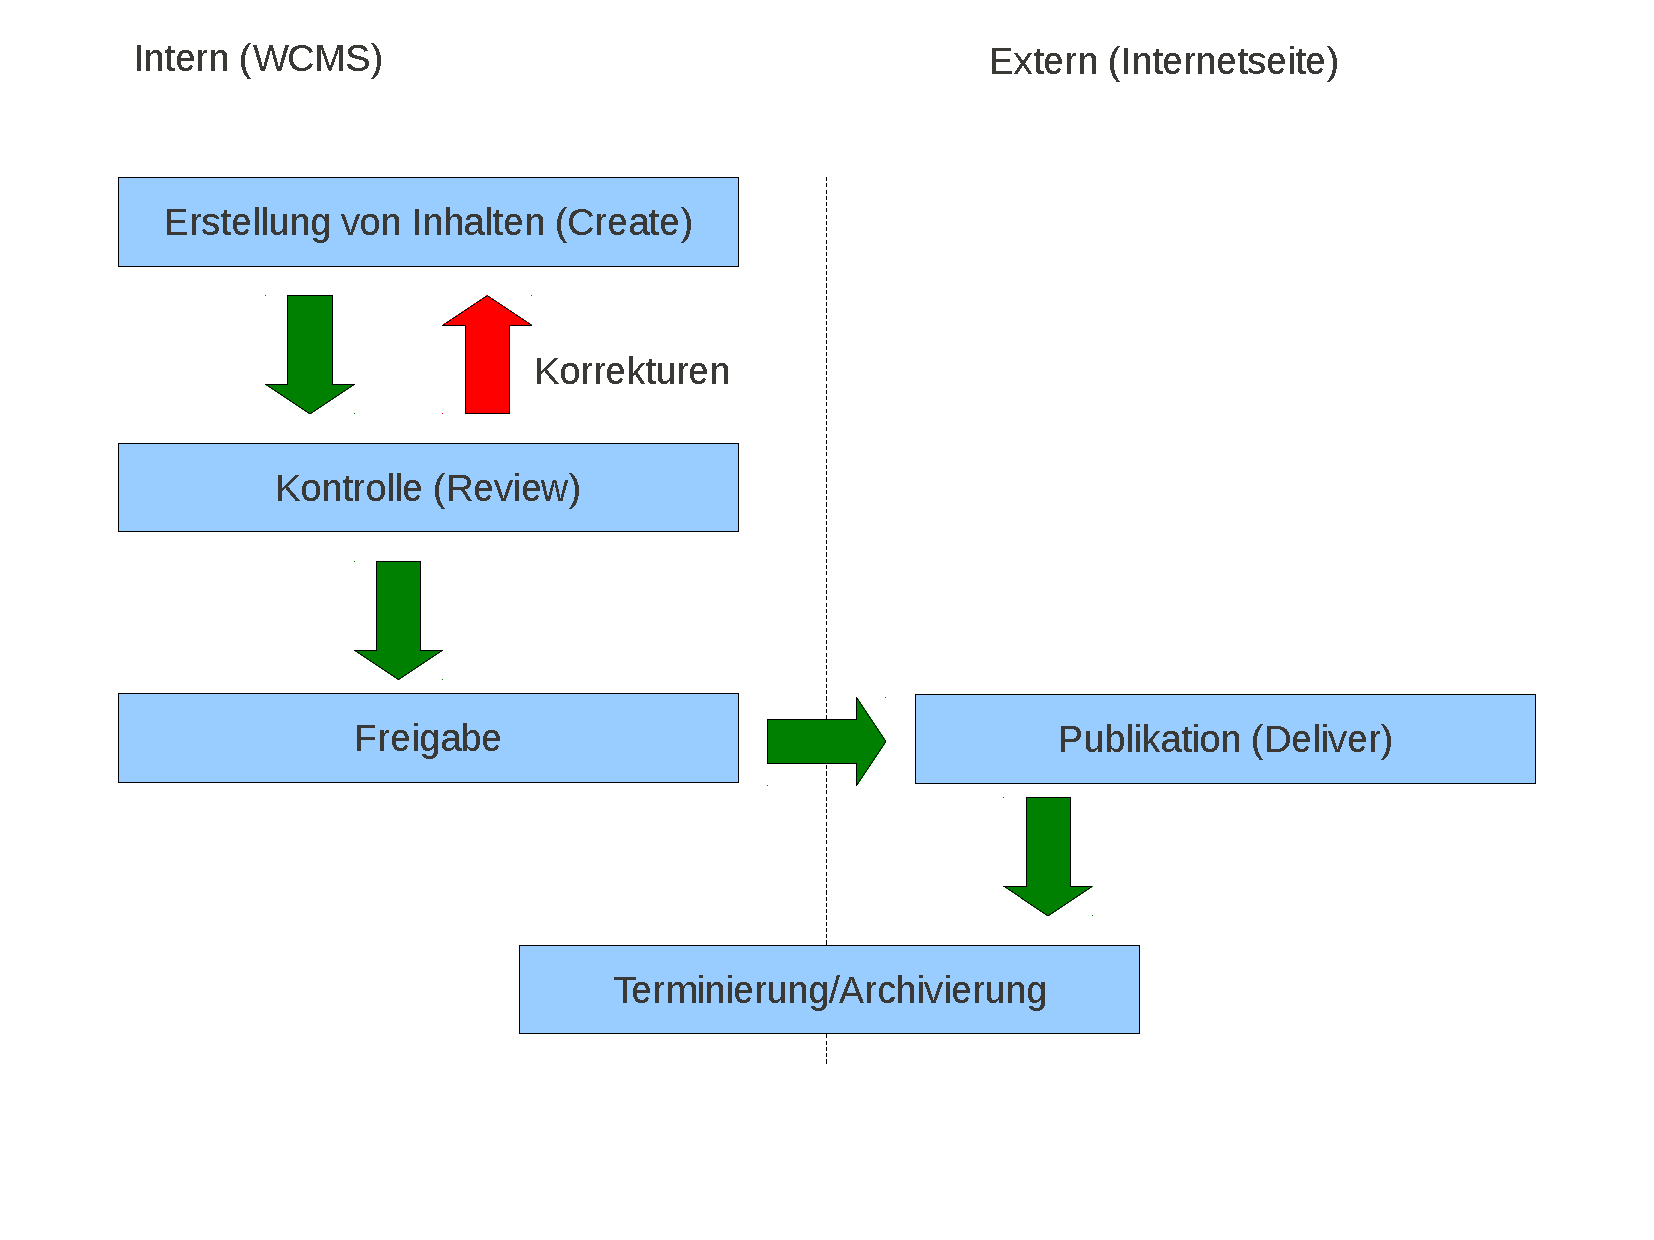
\includegraphics[scale=0.5]{images/grundlagen/lifecycle.pdf}
\caption[Prozessschritte im Content Life Cycle]{Prozessschritte im Content Life Cycle. Eigene Darstellung nach \citep[S. 81]{rockley} und \citep[S. 10]{RitterSwot}}
\label{lifecylcepic}
\end{center}
\end{figure}


\begin{description}
\item[Erstellung]\mbox{~}\\*
Autoren oder Benutzer erzeugen die Inhalte einer Internetseite an Hand der vorliegenden digitalen, (audio-)visuellen Medien oder anderer Informationsträger.
\item[Freigabe und Kontrolle]\mbox{~}\\*
Die Kontrolle von Content schließt sich dem Teilprozess der Content-Erstellung an und stellt durch verschiedene Redakteure und Arbeitsabläufe (Workflows) die Qualität der Inhalte, die auf der Internetseite veröffentlicht werden sollen, sicher. Die Komplexität der Kontrollinstanzen kann dabei unterschiedlich ausgeprägt sein und muss den tatsächlichen Gegebenheiten angepasst werden. Erfüllt der Content die inhaltlichen und gestalterischen Anforderungen nicht, muss dieser von den Autoren erneut überarbeitet werden.
\item[Publikation]\mbox{~}\\*
Nach erfolgter Freigabe des Content erfolgt im Teilprozess Publikation die Veröffentlichung auf der Internetseite. Damit werden die bis dato ausschließlich internen Informationen externen Nutzern zugänglich gemacht. Die eingesetzten WCMS unterscheiden dabei häufig zwischen eine Inter-, Intra- oder Extranetveröffentlichung, welche die Erreichbarkeit der Inhalte auf bestimmte  Zielgruppen einschränkt.
\item[Terminierung und Archivierung]\mbox{~}\\*
Nach Verwendung des Content auf der Internetseite werden bestimmte Inhalte mit steigendem Alter uninteressant oder überflüssig (abhängig von der Art des Inhalts). Durch Aufnahme in ein internes oder öffentliches Archiv können diese für eine spätere Nutzung bzw. Wiederverwendung aufbewahrt werden.
\end{description}

Hauptziel dieses gesamten Redaktionsprozesses ist die Veröffentlichung des Content auf verschiedenen Internetseiten. Der Content Life Cycle bildet somit die wichtigsten Komponenten zur Umsetzung von Web-Publishing, dem Publizieren von Inhalten verschiedenster Medien im Internet, ab. Im folgenden Abschnitt wird der für die funktionale Analyse verwendetet Kriterienkatalog vorgestellt. Dabei werden die formulierten Funktionsbeschreibungen nach den Teilprozessen des Content Life Cycle unterteilt.

\section{Kriterienkatalog}
Die hohe Zahl am Markt befindlicher Web Content Management Systeme führt zu einem erschwerten Auswahlverfahren. Neben kommerziellen WCMS-Lösungen stehen durch die Open Source Bewegung zusätzlich zahlreiche kostenlose Softwareprodukte zur Verfügung, die sich in ihrer Leistungsfähigkeit stark unterscheiden. So kommt es häufig vor, das klein angelegte Open Source Projekte ihre Software stolz als Web Content Management System bezeichnen, obwohl nur sehr wenige Funktionalitäten implementiert sind. Um dieser Praktik entgegenzuwirken, haben Vertreter der Content Management Branche eine Feature-Matrix (Abb. \ref{featurematrix}) herausgegeben, die aktuelle Anforderungen an ein Content Management System spezifizieren soll. Die dabei entstandene Übersicht zeigt dabei eine Unterscheidung in 3 Prioritätsstufen:
\begin{description}
\item[Must-Have]\mbox{~}\\*
Diese Funktionalität muss in einem Web Content Management System verhanden sein.
\item[Should-Have]\mbox{~}\\*
Diese Funktionalität ist nicht zwingend notwendig, kann bei entsprechender Existenz aber sehr positv wahrgenommen werden.
\item[Nice-to-Have]\mbox{~}\\*
Funktionalitäten, die nur in wenigen, hochwertigen Systemen zur Verfügung stehen und über die gewöhnlichen Anforderungen hinausgehen.
\end{description}


\begin{figure}[!h]
\begin{center}
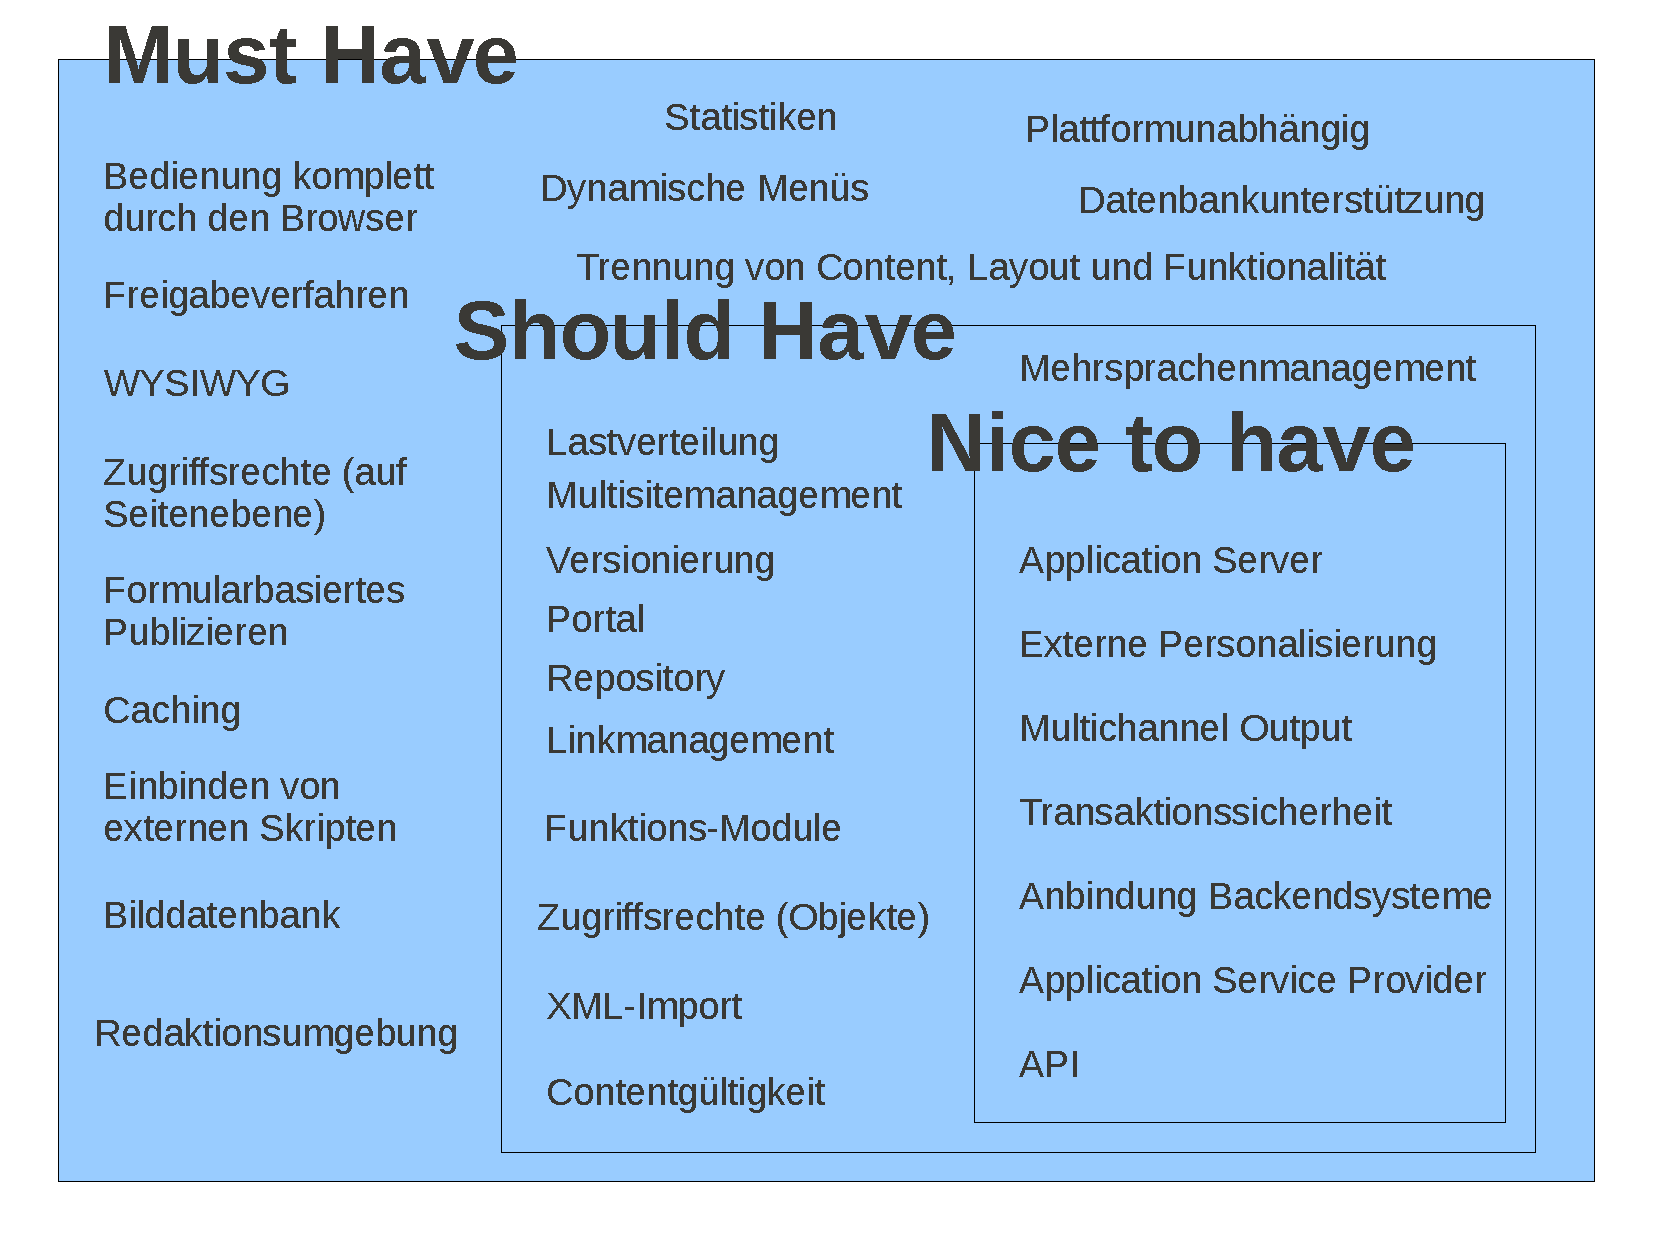
\includegraphics[scale=0.5]{images/analyse/featurematrix.pdf}
\caption[Feature-Matrix für Web Content Management Systeme]{Feature-Matrix für Web Content Management Systeme. Quelle: Eigene Darstellung nach \citep{jdkmatrix}.}
\label{featurematrix}
\end{center}
\end{figure}

Die beschriebenen Funktionalitäten sind jedoch teilweise so allgemein formuliert, das dieser Ansatz nur als grobe Orientierungshilfe dienen kann. Der Wirtschaftsinformatiker Andreas Ritter hat daher im Rahmen seiner Bachelorarbeit \emph{SWOT-Analyse zu Content-Management-Systemen} \cite{RitterSwot} Bereichskriterien erarbeitet, an Hand deren die Leistungsfähigkeit von Web Content Management Systemen untersucht werden kann \citep[][Seite 21-23]{RitterSwot}. Auf Grundlage dieser Bereichskriterien und der afugeführten WCMS-Featurematrix wird in den Kapiteln \ref{sec:erstellung} bis \ref{sec:archi} ein Kriterienkatalog vorgestellt, der allgemeine Funktionalitätsanforderungen unterteilt nach den einzelnen Teilprozessen des Content Life Cycle (Erstellung, Kontrolle, Freigabe, Publikation, Archivierung) formuliert.

\subsection{Erstellung}
\label{sec:erstellung}
\begin{itemize}
\item
In einem WCMS sollen mehrere Redakteure Inhalte gleichzeitig erstellen, ändern, löschen und verwalten können.
\item
In einem WCMS sollen Inhalte – unabhängig von Zeit und Standort – durch mehrere Benutzer online verwaltet und erfasst werden können.
\item
In einem WCMS soll eine Offline-Erfassung von Inhalten unter Verwendung eines lokal auf dem Rechner installierten Programms möglich sein.
\item
Das WCMS verfügt über eine integrierte Mediendatenbank zur Erfassung und Verwaltung von Bildern, Multimedia, Texten, Audio, Videos, usw. Die Inhalte werden dabei in einer Datenbank gespeichert.
\item
Inhalte sollen in einem WCMS ohne spezielle Programmier- und HTML-Kenntnisse erfasst und verwaltet werden können.
\item
Die Nutzung des WCMS erfolgt über einen Internet-Browser. Dabei können alle gängigen Internet-Browser (Internet Explorer, Safari und Firefox) eingesetzt werden.
\item
Ein WCMS soll Inhalte mehrsprachig erfassen und verwalten können.
\item
Inhalte können in einem WCMS während der Erfassung über eine Preview-Funktion vorab im Design der Webseite betrachtet werden.
\item
Das WCMS ermöglicht eine Zuordnung von standardisierten und frei definierbaren Metadaten zu beliebigen Inhalten (z.B. Autor, Schlüsselwörter, benutzerdefinierte Felder).
\item
Das CMS soll über eine offene API (Programmierschnittstelle) für individuelle Erweiterungen verfügen.
\item
Das WCMS ermöglicht die Integration von Inhalten anderer Webseiten, Applikationen oder E-Commerce- Tools.
\item
In einem WCMS sollen Inhalte einfach importiert und exportiert werden können. Beim Austausch kommen Formate wie z.B. XML zum Einsatz.
\end{itemize}



%#### end Erstellung

\subsection{Kontrolle}


\begin{itemize}
\item
Das WCMS verfügt über ein granulares Rechte- und Rollenkonzept für Anwender, Inhalte, Module (Plugins) und Webseiten.
\item
Das WCMS ermöglicht die Versionierung von Inhalten. Zusätzlich können vorhergehende Zustände/Versionen mit Hilfe einer Wiederherstellungsfunktion rekonstruiert werden.
\item
Das WCMS bietet einen Schutz vor gegenseitigem Überschreiben erfasster Inhalte durch z.B. Check in/ Check out- Mechanismen.
\item
Das WCMS ist mandantenfähig, d.h. eine Mehrfachnutzung des Systems durch verschiedene Parteien mit kompletter Trennung der Daten und Benutzer ist möglich.
\item
Das WCMS bietet eine Linküberprüfung, die eine korrekte Darstellung von internen und externen Links auf der Internetseite sicherstellt.
\end{itemize}

%######## end kontrolle

\subsection{Freigabe}

\begin{itemize}
\item
Mit Hilfe des WCMS können \emph{nicht technische} User den Workflowprozesse kreieren, verwalten und ändern. Es sollen dafür keine Programmierkenntnisse notwendig sein.
\item
Das WCMS bildet einen mehrstufigen Workflowprozess für die Freischaltung von Inhalten ab.
\item
Das WCMS bietet die Möglichkeit, externe Mitarbeiter in Workflowprozesse einzubinden.
\item
Unternehmensspezifische Bearbeitungsprozesse von Inhalten sollen über frei definierbare Workflows verwaltet werden können.
\end{itemize}

%##### end freigabe


\subsection{Publikation}

\begin{itemize}
\item
Das WCMS trennt Inhalt und Design durch die Verwendung von Templates.
\item
Das WCMS erlaubt die Mehrfachverwendung von Inhalten an verschiedenen Stellen (auf unterschiedlichen Seiten). Zusätzlich können angelegte Seiten kopiert werden.
\item
Navigationsstrukturen werden vom WCMS automatisch generiert, publiziert und verwaltet.
\item
Die vom WCMS erstellten Seiten können barriefrei umgesetzt werden.
\item
Inhalte sollen vom WCMS auf verschiedene Medien / Technologien (Cross Media Publishing, SMS / Mobile / WAP / usw.) ausgegeben werden können.
\item
Das WCMS bietet Möglichkeiten, Inhalte für anderen Webseiten bereitzustellen (z.B. XML, Webservice).
\item
Das WCMS ermöglicht die Wahl zwischen dynamischer oder statischer Generierung der Seiten bzw. Inhalte (Caching).
\item
Das WCMS unterstützt die automatische Erstellung einer Druckversion für jede einzelne Seite.
\end{itemize}

%############## end publikation

\subsection{Terminierung und Archivierung}
\label{sec:archi}
\begin{itemize}
\item
Das WCMS erlaubt die freie Wahl des Publikationszeitraumes (zeitgesteuertes Auf- / Abschalten / Archivieren) von Inhalten.
\item
Im WCMS können Inhalte und Seiten archiviert werden.
\item
Das WCMS ermöglicht eine Durchsuchung der archivierten Inhalte und Seiten nach wählbaren Parametern (z.B. Monat oder Jahr).
\end{itemize}

%############## end terminierung

